\chapter{Análise Exploratória de Dados}\label{eda}

A análise exploratória de dados, mais conhecida como \textit{Exploratory Data
Analysis} (\textit{EDA}), são procedimentos para a análise de dados, técnicas
para a interpretação dos resultados de tais procedimentos, formas de
planejamento da coleta de dados para fazer a sua análise mais fácil, mais precisa
e mais acurada, e todo o maquinário e resultados estatísticos que se aplicam aos
dados \cite{tukey:1961}. A análise exploratória de dados traz uma variedade de
técnicas para, por exemplo, encontrar características escondidas dos dados,
extrair variáveis importantes e detectar anomalias e \textit{outliers}, sendo
\textit{outlier} um número que é muito maior ou menor que o resto dos números em
uma dada série de números \cite{hawkins80}. Segundo \citeonline{wasiak:2012},
o principal objetivo da abordagem de análise exploratória de dados é adiar as
premissas habituais sobre que tipo de modelo os dados seguem com uma abordagem
mais direta de permitir que os dados revelem a sua estrutura e o modelo.

Para apresentar a análise de dados exploratória foi feita uma rápida comparação
com outros métodos de análise de dados, sendo eles as análises clássica e
bayesiana. A Figura \ref{fig:analysis_comparacao} apresenta um diagrama de
sequência de atividades dos métodos de análises de dados que aqui serão
comparados.

\begin{figure}[h]
  \centering
  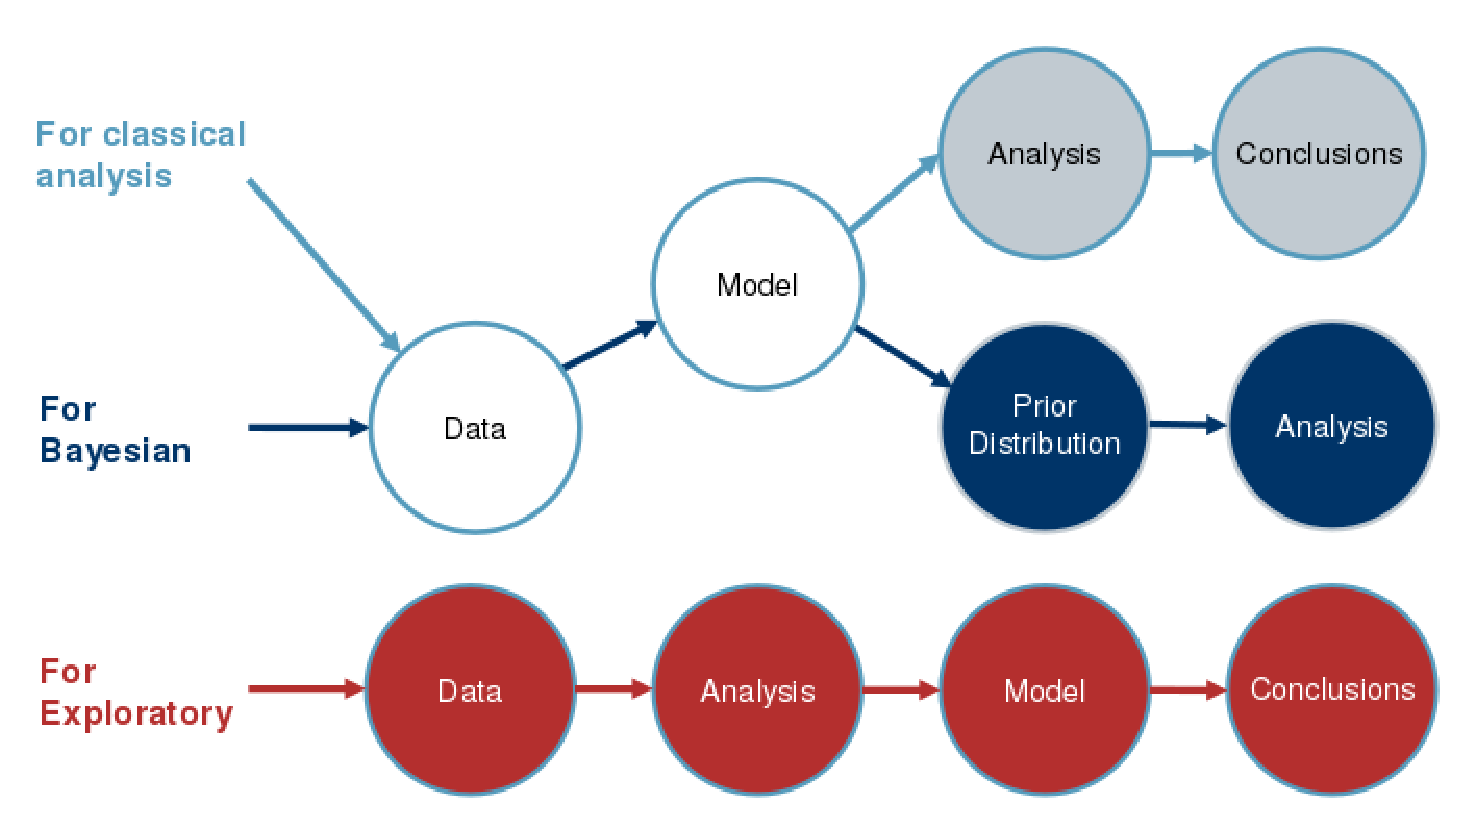
\includegraphics[width=1.0\textwidth]
      {figuras/analysis_comparacao}
      \caption{Diagrama de sequêcia de atividades dos diferente métodos de
      análise de dados \cite{wasiak:2012}}
  \label{fig:analysis_comparacao}
\end{figure}

Como pode-se ver na sequência de atividades apresentadas na Figura
\ref{fig:analysis_comparacao}, os métodos clássico e bayesiano tendem a definir
um modelo para os dados antes de realizar qualquer tipo de análise, a análise é
feita apenas após a definição do modelo, esse tipo de abordagem pode levar a
elaboração de modelos não satisfatórios e isso só será identificado após a
análise desse modelo construído. Esse tipo de erro torna o processo de definição
de um modelos bastante custoso, onde deverá ser realizado o processo de análise
várias vezes até atingir um resultado satisfatório. Já a abordagem de análise
exploratória de dados, como foi dito anteriormente no início do capítulo, visa a
exploração dos dados antes da definição do modelo, deixando os dados
apresentarem as suas estruturas e qual possível modelo melhor se adequa àqueles
dados.

Para a realização dessa análise exploratória dos dados antes da definição de um
modelo são utilizadas vários tipos de técnicas gráficas, tornando-as muito
importante dentro do processo.
